\documentclass[11pt,a4paper]{article}

\usepackage[T1]{fontenc}
\usepackage[utf8]{inputenc}
\usepackage[italian]{babel}
\usepackage{amsmath,amssymb}
\usepackage[a4paper,margin=2.5cm]{geometry}
\usepackage{array}
\usepackage{siunitx}
\usepackage{booktabs}
\usepackage{graphicx}
\usepackage{float}
\usepackage{hyperref}

\hypersetup{hidelinks}
\setlength{\parindent}{0pt}
\setlength{\parskip}{4pt}
\allowdisplaybreaks
\graphicspath{{figure/}}
\sisetup{output-decimal-marker={,}, group-separator={\,}, per-mode=symbol,
         exponent-product=\cdot, range-phrase={\text{--}}}

\newcommand{\uma}{u-a}
\newcommand{\upa}{u+a}
\newcommand{\Mr}{M_{r}}
\newcommand{\fa}{f_a}

\title{Gasdinamica -- Svolgimento esercizio 2\\[2pt]
\large Urto piano contro una brusca riduzione d'area}
\author{}
\date{Prova dell'8/09/2022}

\begin{document}
\maketitle

\section*{Traccia}
Un'onda d'urto piana a $M=3$ propaga in aria in quiete [$\rho_0=\SI{1.29}{kg/m^3}$, $p_0=\SI{1}{atm}$] lungo
un condotto assialsimmetrico nel quale è presente una brusca riduzione dell'area della sezione.
Nell'interazione con la variazione d'area l'urto subisce un fenomeno di riflessione-trasmissione e questo a
sua volta induce la nascita di altre onde. Nelle figure sono riportati i valori assunti lungo il condotto per
diversi istanti di tempo dal numero di Mach e dal fattore di amplificazione
\[
  \fa=\frac{p_5-p_0}{p_1-p_0}.
\]
Fornire una ricostruzione delle caratteristiche principali del flusso generato dall'interazione tra urto e
variazione di sezione. Descrivere il fenomeno nel piano $x$--$t$. (Valutazione 9/30.)

\begin{figure}[H]
  \centering
  \begin{minipage}[c]{0.58\textwidth}\centering
    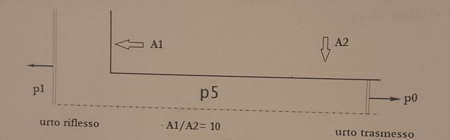
\includegraphics[width=\textwidth]{schema.png}
  \end{minipage}\hfill
  \begin{minipage}[c]{0.38\textwidth}\centering
    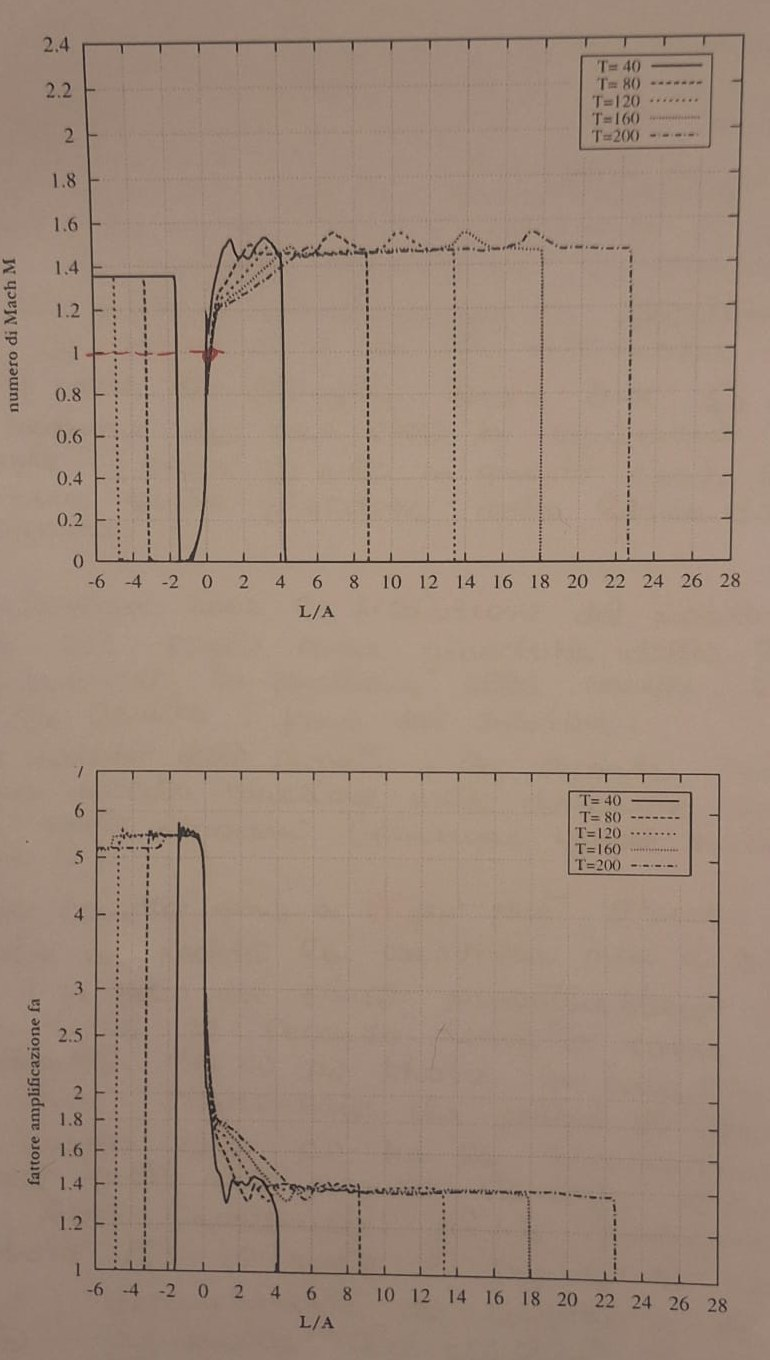
\includegraphics[width=\textwidth]{figure_traccia.jpg}
  \end{minipage}
  \caption{Schema e figure della traccia: condotto largo $A_1$ a sinistra, condotto stretto $A_2$ a destra,
  $A_1/A_2=10$; profili di $M$ e di $\fa$ (scala logaritmica) contro $L/A$ agli istanti $T=40$, 80, 120, 160,
  200.}
  \label{fig:traccia}
\end{figure}

%==============================================================================
\section{Lettura del testo e delle figure}
L'urto incidente viaggia verso destra nel condotto largo $A_1$ e incontra il salto d'area verso il condotto
stretto $A_2=A_1/10$. Dallo schema: $p_0$ è il gas in quiete, $p_1$ lo stato dietro l'urto incidente (cioè
davanti all'urto riflesso, che risale verso sinistra), $p_5$ lo stato dietro l'urto trasmesso. Il fattore
$\fa$ confronta la sovrappressione di ogni punto con quella dell'urto incidente: $\fa>1$ vuol dire
amplificazione.

Le figure sono profili lungo l'asse del condotto, a cinque istanti, del numero di Mach $M=u/a$ e di $\fa$ (asse
in scala logaritmica, da 1 a 7): risultati di un calcolo numerico instazionario. Ascissa $L/A$ e tempo $T$ sono
adimensionali, con il salto d'area in $L/A=0$: i rapporti fra velocità si leggono direttamente, le
velocità assolute no. Nel grafico di $\fa$ i tratti con $\fa<1$ (il gas in quiete, $\fa=0$) escono dal
riquadro. Si chiede di riconoscere le onde, di spiegarne la natura e di ricostruire il piano $x$--$t$.

\begin{table}[H]
  \centering
  \begin{tabular}{lll}
    \toprule
    Grandezza & Valore & Note \\
    \midrule
    $\gamma$, $R$ & $\num{1.4}$, \SI{287}{J/(kg.K)} & aria, gas perfetto \\
    $p_0$, $\rho_0$ & \SI{1}{atm}, \SI{1.29}{kg/m^3} & gas in quiete, $u_0=0$ \\
    $a_0=\sqrt{\gamma p_0/\rho_0}$ & \SI{331.6}{m/s} & $T_0=p_0/(\rho_0R)=\SI{273.7}{K}$ \\
    $M_s$ & 3 & urto incidente \\
    $A_1/A_2$ & 10 & riduzione brusca \\
    \bottomrule
  \end{tabular}
\end{table}

%==============================================================================
\section{Identificazione delle strutture}
Percorro i profili da sinistra a destra (figura~\ref{fig:annotate}).
\begin{enumerate}
  \item \textbf{Stato 1}: $M\approx\num{1.35}$, $\fa=1$. È il gas messo in moto dall'urto incidente, che si
    muove verso il salto d'area con velocità \emph{supersonica}.
  \item \textbf{Urto riflesso}: salto verticale in cui $M$ crolla da \num{1.35} a quasi zero e $\fa$ sale a circa
    \num{5.3}. La sua posizione si sposta verso sinistra con il tempo: è un urto della famiglia $\uma$, che
    risale la corrente supersonica.
  \item \textbf{Stato 2}: gas quasi fermo e ad alta pressione nel condotto largo, fino al salto d'area.
  \item \textbf{Sezione sonica}: nel raccordo il gas accelera e $M$ passa per 1 proprio in $L/A\approx0$, mentre
    $\fa$ scende a circa \num{2.6}. Il salto d'area si comporta come la gola di un ugello alimentato dallo stato 2.
  \item \textbf{Espansione $\uma$}: subito a valle $M$ continua a crescere fino a circa \num{1.46} e $\fa$ scende
    con continuità fino al plateau. La regione di raccordo si allarga in proporzione al tempo e parte sempre da
    $L/A=0$: è un ventaglio centrato nel punto d'incontro urto--salto d'area, con la testa ferma nella sezione
    sonica.
  \item \textbf{Stati 4 e 5, contatto}: plateau con $M\approx\num{1.46}$ e $\fa\approx\num{1.38}$. Sul plateau di $M$
    c'è un piccolo massimo che avanza nel tempo più lentamente dell'urto, mentre nel profilo di $\fa$ nello
    stesso punto non succede nulla: varia la temperatura e non la pressione, quindi è il \textbf{contatto} fra
    il gas passato dal salto d'area (4) e quello che era già nel condotto stretto (5).
  \item \textbf{Urto trasmesso}: salto verticale in testa al plateau, che avanza verso destra. Davanti c'è il gas
    in quiete (0).
\end{enumerate}
Fisico o artefatto: le piccole oscillazioni dietro gli urti e l'ampiezza dei massimi di $M$ sul contatto
(un contatto ideale è un salto netto, non un picco) sono dovute al calcolo numerico, che allarga le
discontinuità. Il profilo a $T=40$ non è ancora autosimile (doppio massimo di $M$, avvallamento di $\fa$ in
$L/A\approx1$): è il transitorio dell'interazione, mentre i profili successivi hanno tutti la stessa forma
allungata nel tempo.

%==============================================================================
\section{Ipotesi ancorate alle figure}
\begin{itemize}
  \item \textbf{Quasi-1D instazionario, non viscoso, gas perfetto con $\gamma=\num{1.4}$}: le figure riportano
    profili a una sola coordinata e gli urti restano verticali e netti, quindi le onde sono piane e le grandezze
    sono medie sulla sezione. Le temperature raggiunte (fino a circa \SI{1250}{K}) rendono $\gamma$ costante
    un'approssimazione accettabile.
  \item \textbf{Salto d'area attraversato in modo stazionario e isentropico}: nelle figure il raccordo occupa
    meno di un'unità di $L/A$ contro le decine percorse dagli urti, e $M=1$ resta fermo in $L/A\approx0$. Fra
    le sezioni $A_1$ e $A_2$ si conservano quindi portata, entalpia totale ed entropia, cioè vale la legge delle
    aree con $p^0$ e $T^0$ uguali. La sezione $A_2$ sonica è una lettura delle figure, che il calcolo deve
    confermare.
  \item \textbf{Problema autosimile}: tutte le onde partono dall'istante e dal punto in cui l'urto raggiunge il
    salto d'area (le rette $x(T)$ misurate passano per lo stesso punto, \S\,\ref{sec:misure}). A ciascun lato del
    salto la soluzione è una sequenza di stati uniformi, urti, contatti e ventagli centrati.
\end{itemize}

%==============================================================================
\section{Misure sulle figure}\label{sec:misure}
Misurando con il righello le posizioni degli urti e dei massimi di $M$ (contatto) ai diversi istanti:
\begin{table}[H]
  \centering
  \begin{tabular}{lccccc}
    \toprule
    $T$ & 40 & 80 & 120 & 160 & 200 \\
    \midrule
    urto riflesso, $L/A$ & $-1.45$ & $-3.10$ & $-4.72$ & -- & -- \\
    contatto (massimo di $M$), $L/A$ & ($3.3$) & $6.9$ & $10.5$ & $13.9$ & $17.5$ \\
    urto trasmesso, $L/A$ & $4.25$ & $8.76$ & $13.35$ & $17.95$ & $22.59$ \\
    \bottomrule
  \end{tabular}
\end{table}
Le posizioni crescono linearmente con $T$, quindi le onde hanno velocità costante:
\[
  W_t\approx\num{0.115},\qquad u^*\approx\num{0.088},\qquad W_r\approx-\num{0.041}\qquad
  \text{(unità di $L/A$ per unità di $T$)},
\]
e le rette dei due urti, prolungate, tornano a $L/A=0$ per $T\approx3$--\num{5}: le onde nascono nello stesso punto.
I rapporti, indipendenti dalle unità, sono
\[
  \frac{W_r}{W_t}\approx-\num{0.36},\qquad \frac{u^*}{W_t}\approx\num{0.77}.
\]
Livelli letti sui grafici: $M_1\approx\num{1.34}$; $\fa\approx\num{5.3}$--\num{5.5} nello stato 2; $\fa\approx\num{2.6}$ nella
sezione d'ingresso del condotto stretto; plateau $M\approx\num{1.46}$ e $\fa\approx\num{1.38}$.

%==============================================================================
\section{Analisi qualitativa}
\textbf{Perché nasce l'urto riflesso.} Una corrente stazionaria supersonica con $M_1\approx\num{1.36}$ può
attraversare una contrazione solo se $A_1/A_2$ non supera $A/A^*(M_1)\approx\num{1.09}$: con $A_1/A_2=10$ il
gas 1 non può entrare così com'è nel condotto stretto. Il gradino è per il 90\,\% della sezione una parete,
quindi si riflette una compressione della stessa natura dell'incidente; dovendo risalire una corrente
supersonica, è un \textbf{urto} $\uma$, che rende subsonico lo stato 2.

\textbf{Perché la sezione è sonica.} Il gas 2, subsonico e ad alta pressione, accelera nella contrazione verso
un condotto stretto inizialmente a \SI{1}{atm}: la differenza di pressione è tale da portare $A_2$ in condizioni
critiche, come la gola di un ugello alimentato da un serbatoio. Lo conferma la figura ($M=1$ in $L/A=0$).

\textbf{Onde nel condotto stretto.} Il gas che entra fa da pistone sul gas in quiete: urto trasmesso $\upa$ e
contatto. Per raccordare lo stato sonico con lo stato dietro l'urto serve un'onda $\uma$: è un'espansione,
in cui il gas accelera oltre $M=1$, con la testa ($u-a=0$) ferma nella sezione sonica. Mi aspetto un urto
trasmesso più forte dell'incidente, perché in un condotto che si restringe un'onda di compressione si
intensifica: la figura lo conferma ($\fa>1$).

%==============================================================================
\section{Topologia del campo}
Il campo è autosimile con centro nell'arrivo dell'urto sul salto d'area (figura~\ref{fig:xt}).
\begin{itemize}
  \item Prima dell'arrivo: stato 0 davanti all'urto incidente, stato 1 dietro.
  \item Condotto largo: stato 1 | \textbf{urto riflesso} $\uma$ ($W_r<0$) | stato 2, uniforme fino al salto d'area.
  \item Salto d'area: collegamento stazionario $2\to3$, con lo stato 3 sonico nella sezione d'ingresso di $A_2$.
  \item Condotto stretto: \textbf{espansione centrata $\uma$} con testa verticale ($u_3-a_3=0$) e coda
    $u_4-a_4>0$ | stato 4 | \textbf{contatto} ($u^*$) | stato 5 | \textbf{urto trasmesso} $\upa$ ($W_t$) |
    stato 0.
\end{itemize}
Non ci sono zone d'interazione a due famiglie: oltre agli stati uniformi c'è un solo ventaglio, un'onda
semplice con caratteristiche $\uma$ semirette. Lo stato 3 occupa solo la sezione d'ingresso del condotto
stretto.

%==============================================================================
\section{Bilancio equazioni/incognite}
Dati gli stati 0 e 1, le incognite sono le intensità delle tre onde: urto riflesso ($\Mr$), espansione $\uma$
e urto trasmesso ($W_t$). Le equazioni sono la condizione di sezione sonica $M_3=1$ e le due condizioni di
contatto $p_4=p_5$, $u_4=u_5$: tre equazioni per tre incognite. Se $A_2$ non fosse sonica, mancherebbe l'onda
$\uma$ separata nel condotto stretto e resterebbero due incognite ($\Mr$, $W_t$) con le due condizioni di
contatto.

%==============================================================================
\section{Scorciatoie fisiche}
Con $A_2$ sonica, $A_2=A^*$ e il Mach dietro il riflesso si legge dalla legge delle aree con $A_1/A^*=10$, senza
conoscere il condotto stretto. Il problema si \textbf{disaccoppia}: l'urto riflesso dipende solo da $M_2$, e il
condotto stretto diventa un problema di Riemann con stato sinistro 3 noto. Poiché $M_2$ risulta molto piccolo,
il primo tentativo per l'urto riflesso è la riflessione su parete chiusa ($u_2=0$).

%==============================================================================
\section{Calcolo}\label{sec:calcolo}

\subsection{Stato 1 (dietro l'urto incidente)}
\[
  \frac{p_1}{p_0}=\frac{2\gamma M_s^2-(\gamma-1)}{\gamma+1}=\num{10.33},\qquad
  \frac{\rho_1}{\rho_0}=\frac{(\gamma+1)M_s^2}{(\gamma-1)M_s^2+2}=\num{3.857},\qquad
  \frac{T_1}{T_0}=\frac{p_1/p_0}{\rho_1/\rho_0}=\num{2.679},
\]
\[
  W_i=M_sa_0=\SI{995}{m/s},\qquad u_1=W_i\left(1-\frac{\rho_0}{\rho_1}\right)=\SI{737}{m/s},
\]
\[
  a_1=a_0\sqrt{\frac{T_1}{T_0}}=\SI{543}{m/s},\qquad M_1=\frac{u_1}{a_1}=\num{1.36}.
\]
Con $p_1=\SI{10.3}{atm}$, $\rho_1=\SI{4.98}{kg/m^3}$, $T_1=\SI{733}{K}$. Per $M_1=\num{1.36}$ la legge delle aree
dà $A/A^*=\num{1.09}\ll A_1/A_2$: la corrente 1 non attraversa la contrazione, nasce l'urto riflesso.

\subsection{Stato 2 (dietro l'urto riflesso) con $A_2$ sonica}
Con $A_2=A^*$, sul ramo subsonico:
\[
  \frac{A_1}{A^*}=\frac1{M_2}\left[\frac{2}{\gamma+1}\left(1+\delta M_2^2\right)\right]^{\frac{\gamma+1}{2(\gamma-1)}}=10
  \quad\Rightarrow\quad M_2=\num{0.058}.
\]
L'urto riflesso viaggia nel gas 1; il salto di velocità fissa il suo Mach relativo e $a_2$ segue dal
rapporto di pressione:
\[
  \Mr=X+\sqrt{1+X^2},\quad X=\frac{\gamma+1}{4}\,\frac{u_1-u_2}{a_1},
\]
\[
  \frac{a_2}{a_1}=\left[\frac{\gamma+1+(\gamma-1)\,p_2/p_1}{\gamma+1+(\gamma-1)\,p_1/p_2}\right]^{1/2},\qquad
  u_2=M_2\,a_2 .
\]
Poiché $a_2$ dipende da $\Mr$, si itera su $u_2$ partendo dalla riflessione su parete:
\begin{table}[H]
  \centering
  \begin{tabular}{cccccc}
    \toprule
    tentativo & $u_2$ [m/s] & $\Mr$ & $p_2/p_1$ & $a_2$ [m/s] & $M_2a_2$ [m/s] \\
    \midrule
    0 (parete) & 0 & 2,104 & 5,00 & 723,0 & 41,9 \\
    1 & 41,9 & 2,029 & 4,64 & 710,1 & 41,2 \\
    \bottomrule
  \end{tabular}
\end{table}
Al secondo tentativo $u_2$ cambia di meno di \SI{1}{m/s}: il valore è assestato.
\[
  \Mr=\num{2.03},\qquad \frac{p_2}{p_1}=\frac{2\gamma\Mr^2-(\gamma-1)}{\gamma+1}=\num{4.64},
\]
\[
  \frac{\rho_2}{\rho_1}=\frac{(\gamma+1)\Mr^2}{(\gamma-1)\Mr^2+2}=\num{2.71},\qquad
  W_r=u_1-\Mr a_1=\SI{-365}{m/s},
\]
con $p_2=\SI{48.0}{atm}$, $\rho_2=\SI{13.5}{kg/m^3}$, $a_2=\SI{710}{m/s}$, $T_2=\SI{1256}{K}$,
$u_2=\SI{41}{m/s}$. L'urto riflesso risale il condotto largo.

\subsection{Stato 3 (sezione d'ingresso del condotto stretto, sonica)}
Fra 2 e 3 si conservano $p^0$ e $T^0$:
\[
  p^0_2=p_2\left(1+\delta M_2^2\right)^{\frac{\gamma}{\gamma-1}}=\SI{48.1}{atm},\qquad
  p_3=p^0_2\left(\frac{2}{\gamma+1}\right)^{\frac{\gamma}{\gamma-1}}=\SI{25.4}{atm},
\]
\[
  u_3=a_3=a_2\sqrt{\frac{2\left(1+\delta M_2^2\right)}{\gamma+1}}=\SI{649}{m/s},
\]
con $\rho_3=\SI{8.57}{kg/m^3}$ e $T_3=\SI{1047}{K}$.

\subsection{Condotto stretto: problema di Riemann fra 3 (sinistra) e 0 (destra)}
Primo tentativo isentropico sulla velocità del contatto:
\[
  z=\frac{a_0}{a_3}\left(\frac{p_3}{p_0}\right)^{\frac{\gamma-1}{2\gamma}}=\num{0.812},\qquad
  u^{(0)}=\frac{z\,(a_3+\delta u_3)-(a_0-\delta u_0)}{\delta(1+z)}=\SI{828}{m/s}.
\]
Con $u^{(0)}>u_3$ a sinistra c'è un'espansione, con $u^{(0)}>u_0$ a destra un urto:
\[
  p_{\rm sx}=p_3\left[1-\delta\,\frac{u-u_3}{a_3}\right]^{\frac{2\gamma}{\gamma-1}},
\]
\[
  p_{\rm dx}=p_0\left[1+\frac{2\gamma}{\gamma+1}\left(M_t^2-1\right)\right],\quad
  M_t=Y+\sqrt{1+Y^2},\quad Y=\frac{\gamma+1}{4}\,\frac{u-u_0}{a_0}.
\]
\begin{table}[H]
  \centering
  \begin{tabular}{cccc}
    \toprule
    passo & $u$ [m/s] & $p_{\rm sx}$ [atm] & $p_{\rm dx}$ [atm] \\
    \midrule
    0 & 828 & 17,1 & 12,5 \\
    1 & 898 & 14,51 & 14,40 \\
    2 & 900,0 & 14,447 & 14,447 \\
    \bottomrule
  \end{tabular}
\end{table}
Al secondo passo $|p_{\rm sx}-p_{\rm dx}|/p\approx4\cdot10^{-6}$, fisicamente zero. Configurazione RCS:
$u^*=\SI{900}{m/s}$, $p^*=\SI{14.4}{atm}$.

\textbf{Stato 4} (coda dell'espansione, $a+\delta u$ uniforme):
\[
  a_4=a_3-\delta\left(u^*-u_3\right)=\SI{598}{m/s},\qquad
  p_4=p_3\left(\frac{a_4}{a_3}\right)^{\frac{2\gamma}{\gamma-1}}=\SI{14.4}{atm},
\]
\[
  M_4=\num{1.50},\qquad u_4-a_4=\SI{302}{m/s},
\]
con $\rho_4=\SI{5.72}{kg/m^3}$, $T_4=\SI{891}{K}$; la testa del ventaglio ha $u_3-a_3=0$.

\textbf{Stato 5} (dietro l'urto trasmesso):
\[
  M_t=\num{3.54},\qquad \frac{p_5}{p_0}=\frac{2\gamma M_t^2-(\gamma-1)}{\gamma+1}=\num{14.4},
\]
\[
  W_t=M_ta_0=\SI{1174}{m/s},\qquad M_5=\frac{u^*}{a_5}=\num{1.48},
\]
con $\rho_5=\SI{5.53}{kg/m^3}$, $T_5=\SI{922}{K}$.

\subsection{Fattore di amplificazione}
\[
  \fa=\frac{p_5-p_0}{p_1-p_0}=\num{1.44}.
\]
L'urto trasmesso è più forte dell'incidente: $M_s$ passa da 3 a \num{3.54}.

%==============================================================================
\section{Verifiche a posteriori}
\begin{itemize}
  \item Urto incidente: $M_s=3>1$, $s_1/s_0=\num{1.56}>1$. Verificata.
  \item Urto riflesso: $\Mr=\num{2.03}>1$ rispetto al gas 1, $s_2/s_1=\num{1.15}>1$, $W_r<0$ (sta nel condotto
    largo). Verificata.
  \item Stato 2 subsonico ($u_2-a_2<0$): le caratteristiche $\uma$ dal salto d'area raggiungono l'urto riflesso e
    il collegamento stazionario con monte subsonico è lecito. Verificata.
  \item Collegamento stazionario: $\rho_2u_2A_1=\rho_3u_3A_2$ e $T^0_2=T^0_3$. Verificata.
  \item Sezione $A_2$ sonica: l'onda $\uma$ nel condotto stretto è un'espansione ($p_4<p_3$, $u_4>u_3$); con una
    compressione l'ipotesi sarebbe caduta. Verificata.
  \item Espansione tutta nel condotto stretto: testa $u_3-a_3=0$, coda $u_4-a_4>0$. Verificata.
  \item Ordine delle onde nel condotto stretto: coda (\SI{302}{m/s}) $<u^*$ (\SI{900}{m/s}) $<W_t$
    (\SI{1174}{m/s}). Verificata.
  \item Urto trasmesso: $M_t=\num{3.54}>1$, $s_5/s_0=\num{1.88}>1$. Verificata.
  \item Contatto: $p_4=p_5$, $u_4=u_5$, $\rho_4\ne\rho_5$; $a>0$ e $p>0$ ovunque. Verificata.
\end{itemize}

%==============================================================================
\section{Risultati}
\begin{table}[H]
  \centering
  \begin{tabular}{clrrrrrr}
    \toprule
    Stato & Posizione & $p$ [atm] & $\rho$ [kg/m$^3$] & $u$ [m/s] & $a$ [m/s] & $T$ [K] & $M$ \\
    \midrule
    0 & quiete & 1 & 1,29 & 0 & 332 & 274 & 0 \\
    1 & dietro l'incidente & 10,3 & 4,98 & 737 & 543 & 733 & 1,36 \\
    2 & dietro il riflesso ($A_1$) & 48,0 & 13,5 & 41 & 710 & 1256 & 0,058 \\
    3 & ingresso di $A_2$ & 25,4 & 8,57 & 649 & 649 & 1047 & 1 \\
    4 & coda dell'espansione & 14,4 & 5,72 & 900 & 598 & 891 & 1,50 \\
    5 & dietro il trasmesso & 14,4 & 5,53 & 900 & 609 & 922 & 1,48 \\
    \bottomrule
  \end{tabular}
\end{table}
\begin{table}[H]
  \centering
  \begin{tabular}{lll}
    \toprule
    Onda & Velocità nel piano $x$--$t$ & Intensità \\
    \midrule
    urto incidente $\upa$ & $W_i=\SI{995}{m/s}$ & $M_s=3$, $p_1/p_0=\num{10.3}$ \\
    urto riflesso $\uma$ & $W_r=\SI{-365}{m/s}$ & $\Mr=\num{2.03}$, $p_2/p_1=\num{4.64}$ \\
    espansione $\uma$ & testa 0, coda \SI{302}{m/s} & $p_4/p_3=\num{0.57}$ \\
    contatto & $u^*=\SI{900}{m/s}$ & $T_4=\SI{891}{K}$, $T_5=\SI{922}{K}$ \\
    urto trasmesso $\upa$ & $W_t=\SI{1174}{m/s}$ & $M_t=\num{3.54}$, $p_5/p_0=\num{14.4}$ \\
    \midrule
    \multicolumn{3}{l}{Fattore di amplificazione $\fa=(p_5-p_0)/(p_1-p_0)=\num{1.44}$ (dalle figure $\approx\num{1.38}$)} \\
    \bottomrule
  \end{tabular}
\end{table}

%==============================================================================
\section{Rappresentazioni}\label{sec:rappr}

\begin{figure}[H]
  \centering
  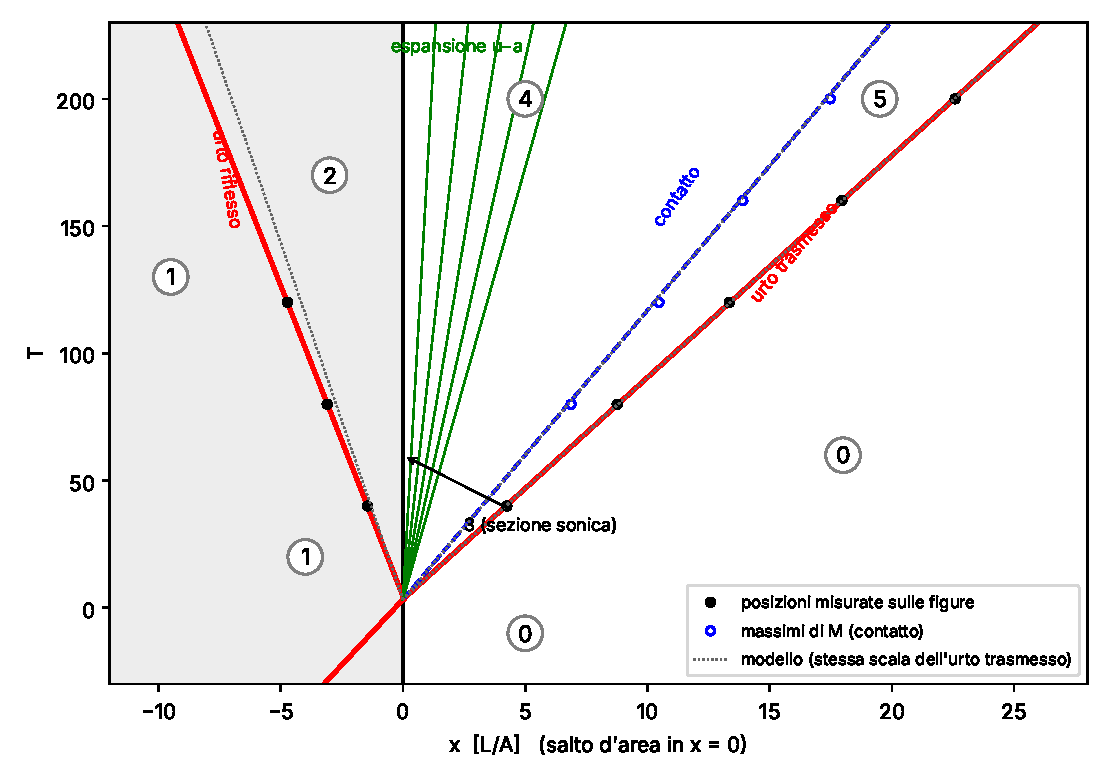
\includegraphics[width=0.85\textwidth]{xt.pdf}
  \caption{Piano $x$--$t$ nelle unità delle figure: posizioni misurate (punti), rette interpolate e
  ventaglio d'espansione; tratteggiate le rette del modello, nella scala che fa coincidere l'urto trasmesso.}
  \label{fig:xt}
\end{figure}
\textbf{Piano $x$--$t$.} Prima dell'arrivo c'è solo l'urto incidente. Dal punto d'arrivo partono tutte le
onde: l'urto riflesso, che risale il condotto largo lasciando dietro di sé il gas 2 quasi fermo; nel condotto
stretto il ventaglio d'espansione con la testa \emph{verticale}, incollata alla sezione sonica, il contatto e
l'urto trasmesso. Le posizioni misurate stanno su rette uscenti dallo stesso punto, come vuole un problema
autosimile; il contatto e l'urto trasmesso del modello coincidono con le misure, l'urto riflesso misurato è un
po' più veloce di quello del modello (discussione al \S\,\ref{sec:coerenza}).

\begin{figure}[H]
  \centering
  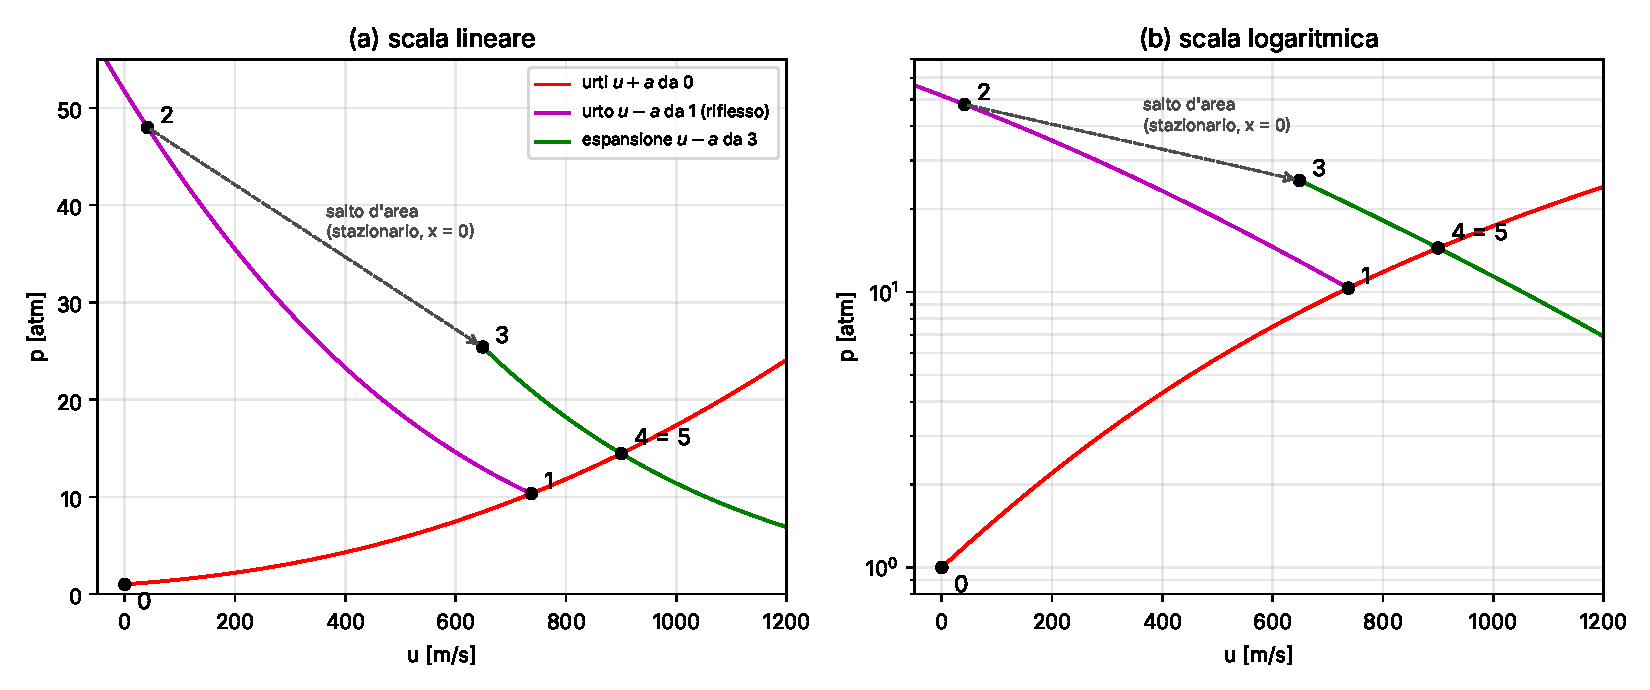
\includegraphics[width=\textwidth]{pu.pdf}
  \caption{Piano $p$--$u$ in scala lineare (a) e logaritmica (b). Il salto $2\to3$ non è un'onda ma il
  collegamento stazionario nella sezione del salto d'area.}
  \label{fig:pu}
\end{figure}
\textbf{Piano $p$--$u$.} Le pressioni vanno da 1 a \SI{48}{atm}, quindi riporto entrambe le scale. Lo stato 1 sta
sulla curva degli urti $\upa$ uscente da 0 (urto incidente). Dal punto 1 lo stato 2 si trova risalendo la curva
dell'urto $\uma$ fino a $u_2\approx0$: è quasi il punto della riflessione su parete. Il salto $2\to3$ avviene
nella sezione del salto d'area e non segue curve d'onda: abbassa la pressione e porta la velocità a quella del
suono. Dal punto 3 la curva d'espansione $\uma$ incontra di nuovo la curva degli urti uscente da 0 nel punto
$4=5$, che sta sopra il punto 1: è l'amplificazione dell'urto. Il contatto non si vede nel piano $p$--$u$
($\rho_4\neq\rho_5$). La scala lineare mostra quanto lo stato 2 sta sopra gli altri; quella logaritmica separa
bene gli stati vicini a $p_0$ e rende leggibili i rapporti di pressione delle singole onde.

\begin{figure}[H]
  \centering
  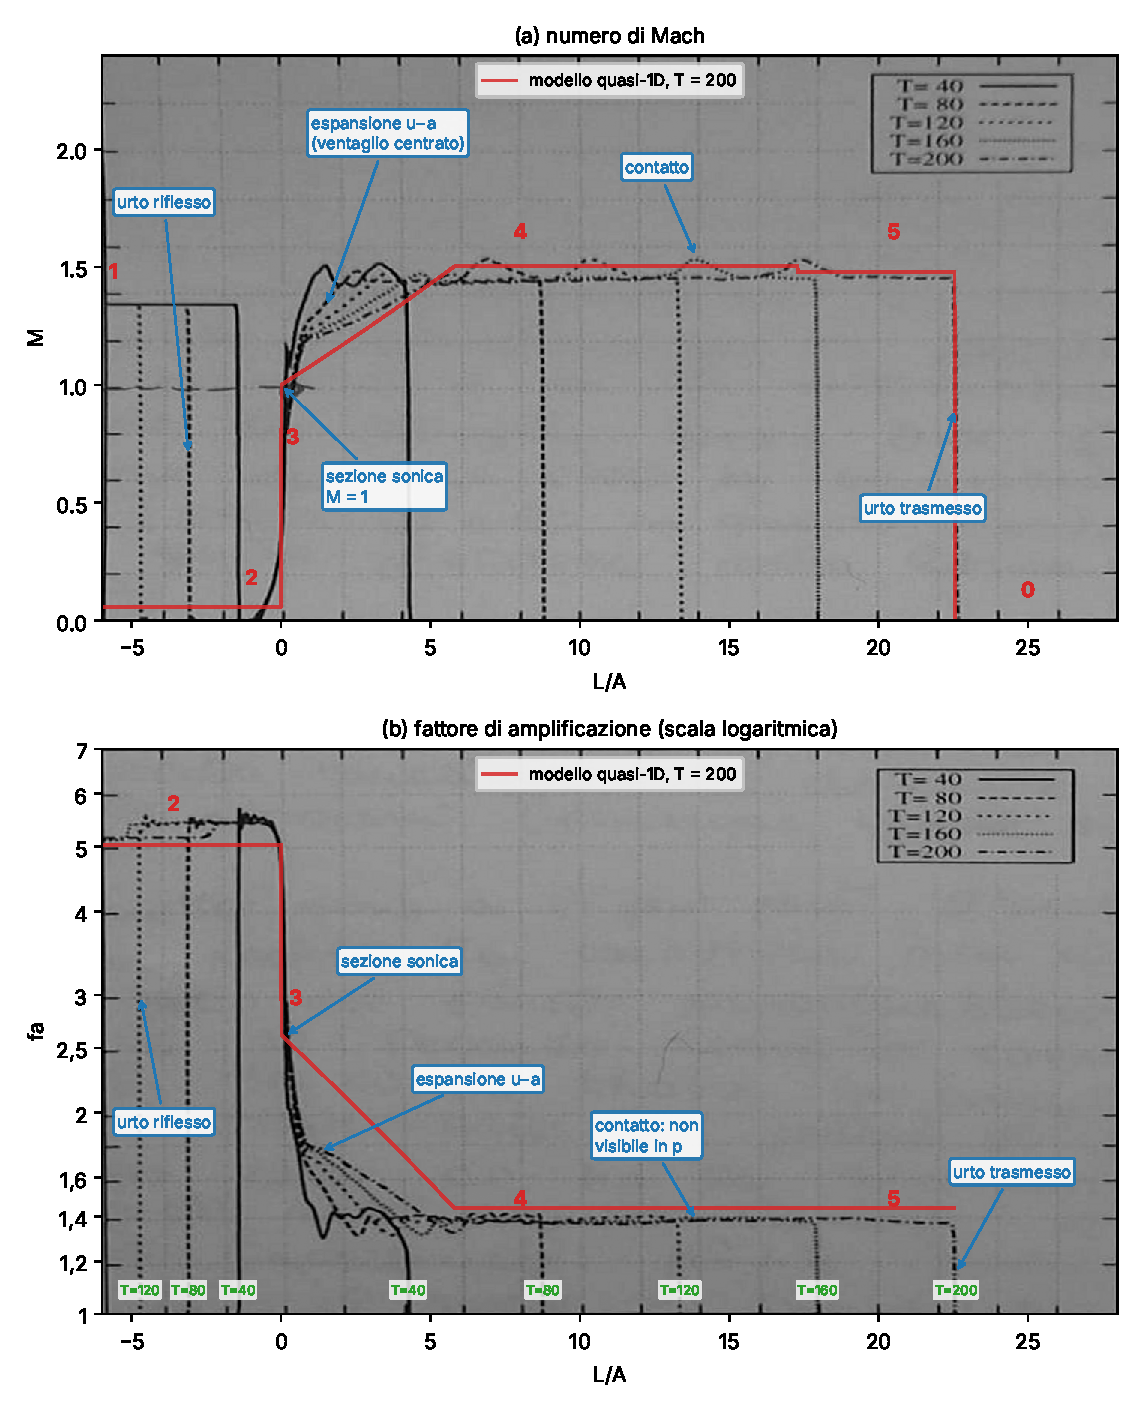
\includegraphics[width=0.92\textwidth]{figure_annotate.pdf}
  \caption{Figure della traccia raddrizzate, con le strutture riconosciute, gli stati e il profilo del modello
  a $T=200$ (in rosso, nella stessa scala del piano $x$--$t$).}
  \label{fig:annotate}
\end{figure}
\textbf{Figure annotate.} Il profilo del modello si sovrappone a quelli della traccia: stessi gradini, stessa
sezione sonica in $L/A=0$, stesso ventaglio e stesso plateau; le differenze di livello sono discusse sotto.

%==============================================================================
\section{Coerenza fra calcolo e figure}\label{sec:coerenza}
\begin{table}[H]
  \centering
  \begin{tabular}{lccc}
    \toprule
    Grandezza & Figure & Modello & Parete chiusa \\
    \midrule
    $M_1$ & \num{1.34} & \num{1.36} & \\
    $\fa$ nello stato 2 & \num{5.3}--\num{5.5} & \num{5.03} & \num{5.43} \\
    $W_r/W_t$ & $-\num{0.36}$ & $-\num{0.31}$ & $-\num{0.35}$ \\
    $M$ nella sezione $A_2$ & 1 & 1 & \\
    $\fa$ nella sezione $A_2$ & \num{2.6} & \num{2.62} & \\
    $M_4$, $M_5$ & \num{1.46} & \num{1.50}, \num{1.48} & \\
    $u^*/W_t$ & \num{0.77} & \num{0.77} & \\
    $\fa$ (plateau) & \num{1.38} & \num{1.44} & \\
    \bottomrule
  \end{tabular}
\end{table}
La struttura coincide: urto riflesso, sezione sonica, ventaglio centrato, contatto visibile solo nel Mach,
urto trasmesso amplificato. Il modello riproduce bene la sezione sonica, il contatto e lo stato 1. Due
differenze sono sistematiche:
\begin{itemize}
  \item \textbf{Condotto stretto}: plateau un po' più basso ($\fa\approx\num{1.38}$ contro \num{1.44}, cioè
    $M_t\approx\num{3.47}$ contro \num{3.54}). Il restringimento reale non è isentropico: allo spigolo vivo
    d'ingresso la corrente si separa (vena contratta) e perde pressione totale. Con una perdita di circa il
    9\,\% ($p^0_3\approx\num{0.91}\,p^0_2$) lo stesso modello dà $\fa=\num{1.38}$ e $M_4\approx M_5\approx\num{1.46}$, come
    le figure.
  \item \textbf{Condotto largo}: l'urto riflesso è più forte del modello ($\fa\approx\num{5.3}$--\num{5.5}, velocità
    $-\num{0.36}\,W_t$) e praticamente uguale a quello su parete chiusa. La perdita lo rinforza di poco
    ($\fa\approx\num{5.07}$); il resto viene dalla corona del gradino, che occupa il 90\,\% della sezione e su cui
    il gas ristagna come su una parete. Il modello quasi-1D, che media sulla sezione e collega 2 e 3 in modo
    ideale, non vede questo effetto bidimensionale.
\end{itemize}

%==============================================================================
\section{Discussione fisica}\label{sec:disc}
\textbf{Perché l'urto si amplifica.} Il salto d'area si comporta come la gola di un ugello alimentato da un
serbatoio: il gas 2, quasi fermo, ha $p^0\approx\SI{48}{atm}$ e $T^0\approx\SI{1256}{K}$ e scarica nel condotto
stretto in condizioni soniche. Il condotto stretto diventa un tubo d'urto con un ``driver'' più caldo e a
pressione più alta dello stato 1, e l'urto trasmesso è più forte dell'incidente.

\textbf{Peso del rapporto d'area.} Con $A_1/A_2=10$ il riflesso è già vicino a quello su parete chiusa. Lo stesso
modello dà $\fa\approx\num{1.20}$ per $A_1/A_2=2$ e $\fa\approx\num{1.52}$ per $A_1/A_2\to\infty$: con un rapporto 10
l'amplificazione è vicina al suo limite. Ogni contrazione con $A_1/A_2>\num{1.09}$ strozza la sezione $A_2$;
solo sotto questo valore la corrente supersonica 1 passerebbe senza urto riflesso.

\textbf{Contatto.} Il gas 4 ha attraversato due urti ($M_s=3$ e $\Mr=\num{2.03}$) e un'espansione, il gas 5 un solo
urto, più forte ($M_t=\num{3.54}$): il gas 5 ha più entropia ed è più caldo, quindi ha velocità del suono
maggiore e, a pari $u$, Mach minore. Per questo il contatto compare come un gradino (nel calcolo numerico un
piccolo picco) nel profilo di $M$ e non in quello di $\fa$.

\textbf{Limiti del modello.} Nei primi istanti il campo è bidimensionale: l'urto incidente si riflette sulla
corona del gradino e diffrange sullo spigolo d'ingresso, e l'urto trasmesso è inizialmente curvo. È il
transitorio visibile nel profilo a $T=40$, non ancora autosimile. Più avanti lo strato limite nel condotto
stretto attenuerebbe gradualmente l'urto trasmesso; nei tempi delle figure il plateau resta costante.

\end{document}
